\documentclass[review]{elsarticle}

\usepackage{lineno,hyperref}
\usepackage[utf8]{inputenc}
\modulolinenumbers[5]

\journal{Renato Vimieiro}

%%%%%%%%%%%%%%%%%%%%%%%
%% Elsevier bibliography styles
%%%%%%%%%%%%%%%%%%%%%%%
%% To change the style, put a % in front of the second line of the current style and
%% remove the % from the second line of the style you would like to use.
%%%%%%%%%%%%%%%%%%%%%%%

%% Numbered
%\bibliographystyle{model1-num-names}

%% Numbered without titles
%\bibliographystyle{model1a-num-names}

%% Harvard
%\bibliographystyle{model2-names.bst}\biboptions{authoryear}

%% Vancouver numbered
%\usepackage{numcompress}\bibliographystyle{model3-num-names}

%% Vancouver name/year
%\usepackage{numcompress}\bibliographystyle{model4-names}\biboptions{authoryear}

%% APA style
%\bibliographystyle{model5-names}\biboptions{authoryear}

%% AMA style
%\usepackage{numcompress}\bibliographystyle{model6-num-names}

%% `Elsevier LaTeX' style
\bibliographystyle{elsarticle-num}
%%%%%%%%%%%%%%%%%%%%%%%

\begin{document}

\begin{frontmatter}

\title{Relatório Projeto Data Science - Reclamações Procon}


%% Group authors per affiliation:
\author{Arthur Bezerra de Freitas}
\author{Leonardo do R�go Esp�ndola}
\author{Matheus Barbosa Domingues Feliciano}
\address{Universidade Federal de Pernambuco � Centro de Inform�tica
\linebreak Caixa Postal 7.851 � 50.732-970 � Recife, PE � Brasil
\linebreak abf2@cin.ufpe.br, lre@cin.ufpe.br, mbdf@cin.ufpe.br}

\begin{abstract}
    O Sistema Nacional de Informações de Defesa do Consumidor – Sindec é um sistema informatizado que integra processos e procedimentos, relativos ao atendimento aos consumidores nos Procons, visando proporcionar um instrumento de gestão. Este trabalho tem como objetivo estudar os dados obtidos pelo sistema das reclamações dos brasileiros à companhias e extrair informações utilizando as abordagens de data science a fim de entender como esse relacionamento entre cliente e fornecedor se dá.
\end{abstract}

\end{frontmatter}

\linenumbers

\section{Introdução}
A partir de dados obtidos através do repositório online dados.gov.br de reclamações do Procon entre os anos de 2009 e 2016 fizemos análises exploratórias relacionando posição geográfica, idade, sexo e outro mais com a resolução da reclamação. Além disso, foram feitas análises de predição de uma reclamação ser atendida ou não, de acordo com alguns desses atributos. Os algoritmos de classificação utilizados foram Árvore de Decisão e Naive Bayes.

\section{Coleta}
A base de dados escolhida para estudo foi coletada no repositório online dados.gov.br e descreve os dados de reclamações fundamentadas feitas por consumidores ao Procon entre os anos de 2009 e 2016. A base contém mais de 100 5 mil reclamações fundamentadas por ano, com informações detalhadas sobre a reclamação, a empresa e informações gerais sobre o consumidor, além de descrever se a reclamação foi atendida ou não, segundo os critérios do Procon. Os dados estão disponíveis em formato CSV separados por arquivos anuais. 

\section{Pré-Processamento}
    Como nossa base tinha um volume muito grande de dados, escolhemos trabalhar somente com o ano de 2016. Numa primeira análise removemos colunas que seriam irrelevantes para a análise dos dados. As colunas removidas foram “AnoCalendario”, “NumeroCNPJ”, “DescCNAEPrincipa”', “RadicalCNPJ”, “RazaoSocialRFB”. Essas colunas traziam informações de identificação das empresas que não eram relevantes, assim como o ano do calendário, que já era descrito pelo csv que escolhemos.

	Após a remoção dessas colunas, nos deparamos com um conjunto de dados com 203.485 linhas e 18 colunas. Como o conjunto ainda estava bastante grande, decidimos remover todas as linhas que tinham valores nulos. Assim reduzimos a quantidade de linhas para 79.515.
	
	O próximo processo feito foi o de converter cada coluna do conjunto de dados para o seu devido tipo. Verificamos que as colunas de “DataArquivamento” e “DataAbertura” deveriam ser o tipo “datetime64”, enquanto as demais foram atribuídas o tipo category. Ou seja, eram colunas categóricas.
	
	Após a definição de tipos das colunas, verificamos que seria interessante termos uma nova coluna “período”, que foi gerada a partir de “DataArquivamento” e “DataAbertura”, sendo definida pela quantidade de dias que a reclamação esteve aberta. Foi atribuído o tipo “float64” para a coluna “período”.
	
	Após a criação da coluna período, a coluna de “FaixaEtariaConsumidor” teve uma categorização ordenada, sendo criada uma nova coluna que definia faixas de idades como: "até 20 anos","entre 21 a 30 anos","entre 31 a 40 anos","entre 41 a 50 anos","entre 51 a 60 anos","entre 61 a 70 anos","mais de 70 anos".
	Por fim, novas colunas que mapeavam os valores categóricos que seriam usados pelos classificadores foram criadas. E além disso, uma nova coluna para definir se o atributo “Venda Enganosa” estava presente ou não naquela linha foi criada para utilização na hipótese 3.

\section{Análise exploratória}

    Na fase inicial da análise construímos alguns gráficos de barra para ter uma melhor noção de como os dados estavam distribuídos na base, estes gráficos estão representados pelas figuras abaixo:

\includegraphics{figura1p1.png}


\includegraphics[width=150mm,scale=1]{figura1p2.png}

 
\includegraphics[width=150mm,scale=1]{figura1p3.png}

 
\includegraphics[width=130mm,scale=0.8]{figura1p4.png}

 \vspace*{5px}
    Como podemos observar, os problemas mais recorrentes são relacionados a contrato, serviço não fornecido e cobrança indevida que bate com as empresas que fornecem produtos através de contratos e cobrança recorrente (mensal) e os assuntos dos problemas geralmente envolvem o mesmo domínio.
    
    Após isso, foram feitas as análises para tentar provar ou refutar, cada uma das hipóteses propostas. Para algumas hipóteses foi somente necessário um gráfico correlacionando os atributos, porém para outras utilizamos algoritmos de classificação para a realização das provas. 

 \vspace*{5px}
 \textbf{Hipótese 1:} \textit{Faixa Etária e Gênero influenciam no número total de reclamações.}
 
 \vspace*{5px}
	A validação dessa hipótese foi feita a partir do agrupamento dos atributos de “FaixaEtariaConsumidor” e “SexoConsumidor” em relação a frequencia de “Atendida” (coluna que definia a situação da reclamação). Como podemos ver na figura 2, temos um número maior de reclamações para pessoas entre 31 e 40 anos, tanto para o sexo masculino quanto para o feminino. Porém, há um número maior de reclamações para o sexo feminino nesta mesma faixa etária.
	
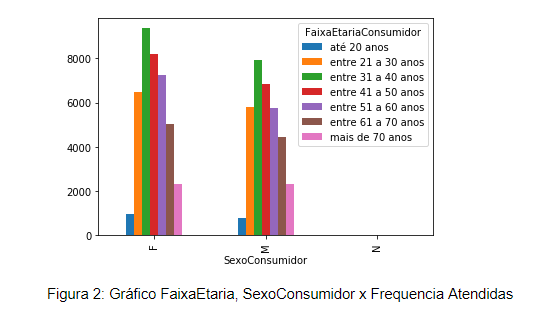
\includegraphics{figura2}

\textbf{Hipótese 2:} \textit{As regiões Norte e Nordeste têm menos resolução de reclamações do que as demais regiões.}

\vspace*{5px}
    Para validar essa hipótese, uma crosstable entre as colunas “Atendida” e “Regiao” definindo a porcentagem de reclamações atendidas ou não para cada uma das regiões. Após a construção dessa crosstable, foi criado um gráfico que demonstrou esses valores em relação à média do conjunto de dados. 
    
    Como podemos ver na figura 3, a hipótese foi refutada, tendo como pior porcentagem de reclamações atendidas a região Sudeste, porém a região Norte vem como segunda pior, ambas abaixo da média de 61\%. Enquanto as demais regiões, todas têm valores de reclamações atendidas acima da média. 

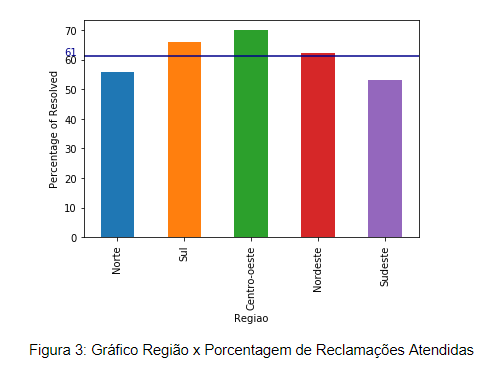
\includegraphics{figura3}
\vspace*{5px}

\textbf{Hipótese 3:} \textit{O sexo do consumidor e faixa etária são determinantes para inferir se a reclamação teve como descrição “Venda Enganosa”.}

\vspace*{5px}
	A validação dessa hipótese foi feita com o uso dos algoritmos de classificação Naive Bayes e Decision Tree. Os atributos escolhidos foram “FaixaEtariaConsumidor” e “SexoConsumidor”. Esses atributos foram devidamente pré-processados, como descrito anteriormente, e então foram usados para prever a nova coluna criada indicando a presença ou não do atributo “Venda Enganosa”. 
	
    Quando executamos pela primeira vez o algoritmo, tivemos um resultado de acurácia próximo de 100\%. Porém, a matriz de confusão, descrita pela figura 6, indicava que os acertos estavam todos sendo feitos para a classe de não Venda Enganosa. Ou seja, como criamos a coluna separando em Sim ou Não para Venda Enganosa, o algoritmo só acertou para o Não. 
    
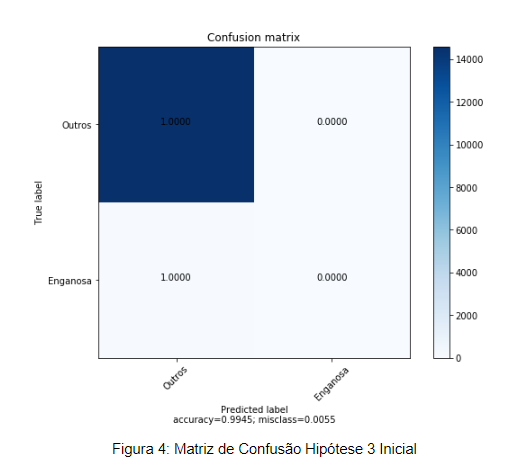
\includegraphics{figura4}

Após verificarmos o conjunto de dados, vimos que o número de instância de Não Venda Enganosa era de 73001, enquanto o de Sim Venda Enganosa era de 412. Portanto, temos uma disparidade na distribuição de classes. 

Para contornar esse problema, utilizamos a técnica de oversampling no conjunto de treinamento. Após o treinamento com oversampling, tivemos os seguintes resultados dos testes de acurácia e mean squared error (MSE) para Naive Bayes e Decision Tree:

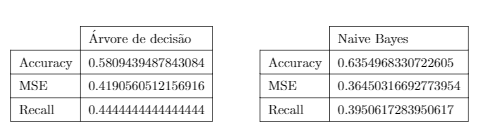
\includegraphics{table1}

Também podemos ver nas matrizes de confusão representadas pelas Figuras 5 e 6, que mesmo após o oversampling esses atributos não tem relevância na definição de Venda Enganosa.

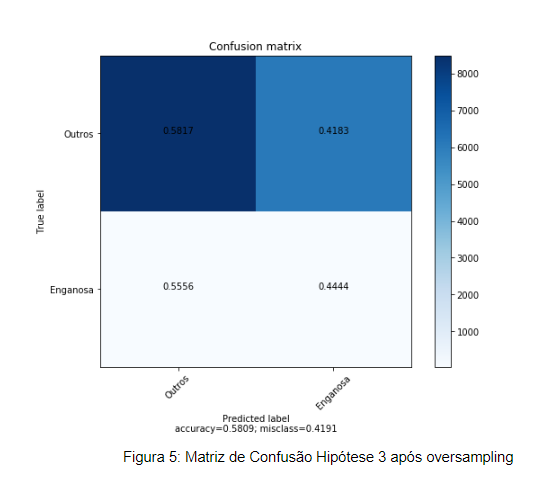
\includegraphics{figura5.png}

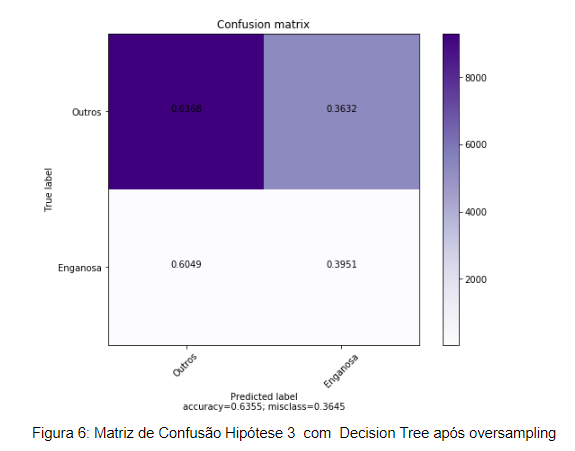
\includegraphics{figura6.png}

\vspace*{5px}

\textbf{Hipótese 4:} \textit{É possível inferir a partir dos atributos categóricos presentes no conjunto de dados, após o pré-processamento, se uma reclamação foi atendida ou não.}

\vspace*{5px}

	A validação dessa hipótese foi feita com o uso de dois algoritmos de classificação: Naive Bayes e Decision Tree. Os atributos escolhidos para serem usados na classificação foram todos os categóricos.
	
	Os atributos de “DataAbertura”, “DataFechamento” e período não seriam interessantes para a classificação, já que o pressuposto para eles existirem é que a reclamação já teve uma resolução de atendida ou não. 
	
	Após dividir o conjunto de dados em treinamento e teste e treinarmos os classificadores, tivemos os seguintes resultados dos testes de accuracy e mean squared error (MSE) para Naive Bayes e Decision Tree:
	
\vspace*{5px}	
	
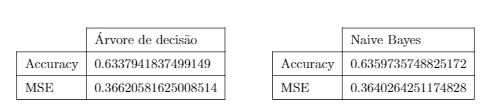
\includegraphics{table2.png}

\vspace*{5px}

Também podemos ver nas matrizes de confusão, descritas pelas Figuras 4 e 5, que o nível de acerto para as reclamações que tiveram a resolução como Atendida é bem maior do que para não atendida.

\vspace*{10px}

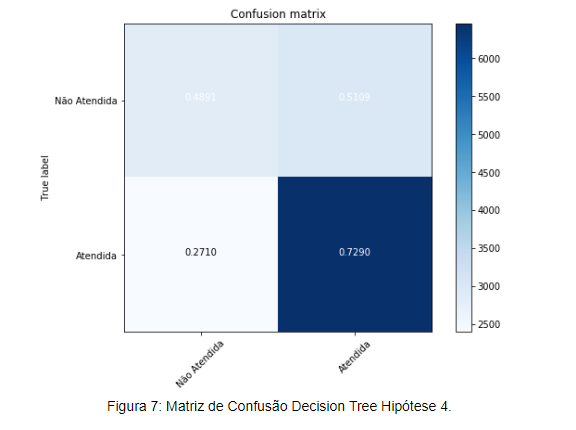
\includegraphics{figura7.png}

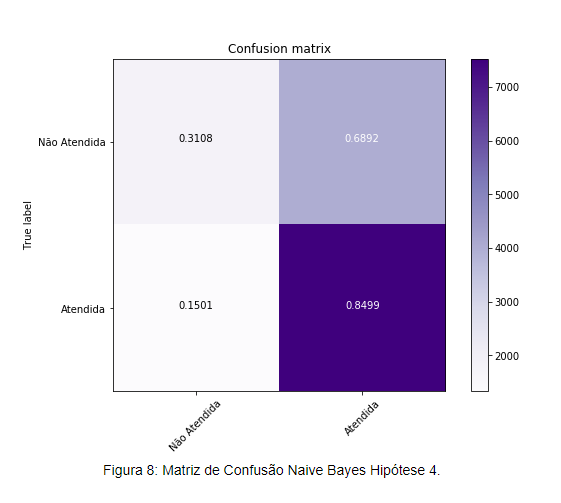
\includegraphics{figura8.png}

\section{Conclusão}
Ao fim da análise dos dados, podemos verificar como verdadeiras algumas das hipóteses que propomos e também nos surpreendemos com alguns dos resultados. A conclusão que podemos tirar é que os dados descrevem bem as resoluções atendidas pelas empresas. Ou seja, conseguimos definir bem, de acordo com as características das reclamações, o que é uma reclamação que será atendida. Porém, já para as reclamações que não são atendidas, temos motivos muito diversos, o que dificulta a definição de um padrão para as reclamações não atendidas.

\end{document}